\documentclass{article}
\usepackage{fullpage,amsmath,amsthm,graphicx,enumitem,amsfonts}
\usepackage{multicol}
\usepackage{booktabs}
\usepackage{algorithm}
\usepackage{algpseudocode}

\usepackage{tikz}
\usetikzlibrary{positioning, shapes, arrows, fit}

\theoremstyle{definition}
\newtheorem{thm}{Theorem}
\newtheorem{question}[thm]{Question}
\newenvironment{solution}{\noindent\textit{Solution:}}{}

\title{ASEN 5264 Decision Making under Uncertainty\\
       Exam 2: Online Methods and Reinforcement Learning}

\date{\small 
    \textbf{Instructions:} Clearly indicate your final answers and briefly justify numerical answers with text or mathematical expressions. If you do not understand how to do a problem, skip it and move on so that you have time to attempt all problems. You may consult any static source, but you may NOT communicate with any person except the instructor or TA, and you may not use LLMs such as ChatGPT.
}

\begin{document}
\maketitle

\noindent\textbf{Important:} Please include the following statement along with your signature (typed or handwritten) on the exam: \textbf{``I affirm that I completed this exam without the use of any artificial intelligence tool such as ChatGPT or Github Copilot.''}

\begin{question} (10 pts)
    Suppose that we are using Q-learning to solve an MDP with $S = \{1, 2\}$ and $A = \{\text{a}, \text{b}\}$. The current Q values are given in the table below:
    \begin{center}
        \begin{tabular}{cc|cc}
            \toprule
            $s$ & $a$ & $Q(s, a)$ \\
            \midrule
            1 & a & 5 \\
            1 & b & 3 \\
            2 & a & 4 \\
            2 & b & 2 \\
            \bottomrule
        \end{tabular}
    \end{center}
    If we take step $(s=1, a=\text{a}, s'=2, r=6)$ and use the Q-learning update rule with $\alpha = 0.1$ and $\gamma = 0.9$, which Q values are changed and what are their new values?
\end{question}

% \begin{question}
% \end{question}

\clearpage

\begin{question} (20 pts)
    Consider a three-armed Bernoulli bandit with win probabilities $\theta = [0.3, 0.7, 0.4]$. After 10 pulls of each arm, the number of wins for each arm is $w = [2, 5, 6]$.
    \begin{enumerate}[label=(\alph*)]
        \item What is the probability that the next pull will result in a win (+1 reward) if an epsilon greedy policy is used with $\epsilon = 0.1$? Briefly justify your answer.
        \item What is the probability that the next pull will result in a win (+1 reward) if a UCB policy is used with $c = 1$? Briefly justify your answer.
        \item After a very large number of pulls, which policy will have the highest average payoff? epsilon-greedy or UCB? Briefly justify your answer.
    \end{enumerate}
\end{question}

\clearpage

\begin{question} (20 pts)
    Consider a candidate reinforcement learning algorithm for MDPs with integer states and actions that keeps track of a large table, $Q$, where each row corresponds to a state and each column to an action. Let $Q[s, a]$ be the entry in row $s$ and column $a$.
    The algorithm works as follows: 
    \\
    \begin{algorithmic}[1]
        \State Initialize $Q$ to be a matrix of zeros.
        \State Initialize $s$ to be the initial state.
        % \State Initialize $R$ to 0.
        \Loop
            \State $a \gets \text{argmax}\, Q[s, a]$ (Break ties randomly).
            \State Take action $a$, receive reward $r$, and observe the next state $s'$.
            \State $Q[s, a] \gets Q[s, a] + 0.1 (r - Q[s, a])$
            \State $s \gets s'$
            \If{$s$ is a terminal state}
                \State Reset $s$ to the initial state.
            \EndIf
        \EndLoop
    \end{algorithmic}

    \begin{enumerate}[label=(\alph*)]
        \item Should this algorithm be considered model-based or model-free? Why?
        \item Should this algorithm be considered on-policy or off-policy? Why?
        \item What is a major limitation of this algorithm related to exploration? Briefly justify your answer.
        \item What is a major limitation of this algorithm related to credit assignment? Briefly justify your answer.
        % ask in a way that narrows their responses
    \end{enumerate}
\end{question}

\clearpage
\begin{question} (20 pts)
    Consider the following MCTS tree where state nodes are represented with circles and action nodes with squares. States are represented with integers and there are two actions, a and b. If the generative function is called at any point, use the values in the table to the right and use a discount of $\gamma=0.9$ if needed.\\
    \\
    \begin{minipage}{0.5\textwidth}
    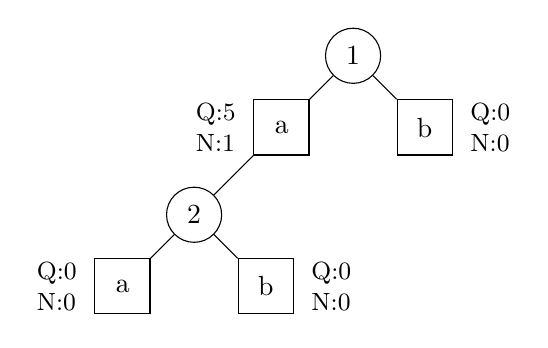
\begin{tikzpicture}
      % Define styles for nodes
      \tikzset{
        circlenode/.style={circle, draw, minimum size=0.7cm, inner sep=0pt},
        squarenode/.style={rectangle, draw, minimum size=0.7cm, inner sep=2pt},
        annotation/.style={font=\small}
      }
      
      % Create the tree structure with the nodes
      \node[circlenode] (node1) {1};
      \node[squarenode, below left=0.3cm and 0.3cm of node1] (nodea1) {a};
      \node[squarenode, below right=0.3cm and 0.3cm of node1] (nodeb1) {b};
      
      \node[circlenode, below left=0.5cm and 0.5cm of nodea1] (node2) {2};
      \node[squarenode, below left=0.3cm and 0.3cm of node2] (nodea2) {a};
      \node[squarenode, below right=0.3cm and 0.3cm of node2] (nodeb2) {b};
      
      % Draw the edges connecting the nodes
      \draw (node1) -- (nodea1);
      \draw (node1) -- (nodeb1);
      \draw (nodea1) -- (node2);
      \draw (node2) -- (nodea2);
      \draw (node2) -- (nodeb2);
      
      % Add annotations next to the nodes
      \node[annotation, left=0.1cm of nodea1, align=left] {Q:5\\N:1};
      \node[annotation, right=0.1cm of nodeb1, align=left] {Q:0\\N:0};
      \node[annotation, left=0.1cm of nodea2, align=left] {Q:0\\N:0};
      \node[annotation, right=0.1cm of nodeb2, align=left] {Q:0\\N:0};
    \end{tikzpicture}
    \end{minipage}
    \begin{minipage}{0.5\textwidth}
        \begin{center}
            G(s, a)\\
            \begin{tabular}{cc|cc}
                \toprule
                $s$ & $a$ & $s'$ & $r$ \\
                \midrule
                1 & a & 2 & 6.0 \\
                1 & b & 3 & 7.0 \\
                2 & a & 4 & 5.0 \\
                2 & b & 4 & 6.0 \\
                \bottomrule
            \end{tabular}
        \end{center}
    \end{minipage}
    \vspace{3cm}
    \begin{enumerate}[label=(\alph*)]
        \item Suppose we run one iteration of MCTS starting from node 1. What is the path of states and actions that the search phase will take including any new state nodes created (e.g. (1, b, 2, b, 5) or (1, a, 4))? Briefly justify why each node is selected.
        \item Draw any new state and action nodes that would be created in the expansion phase (you can either add to the existing tree or re-draw the tree).
        \item Assume the rollout from the new leaf node returns a value estimate of 10. Perform the backup to update the Q and N values at all action nodes nodes on the path (you do not need to copy unchanged values from the existing tree).
    \end{enumerate}
\end{question}



\end{document}
